\documentclass{standalone}
\usepackage{tikz}
\usepackage{ctex,siunitx}
\usepackage{tkz-euclide}
\usepackage{amsmath}
\usetikzlibrary{patterns, calc}
\usetikzlibrary {decorations.pathmorphing, decorations.pathreplacing, decorations.shapes,}
\begin{document}
\small
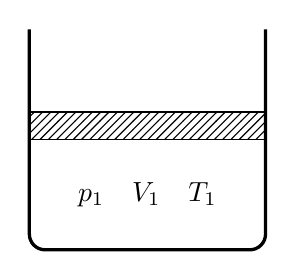
\begin{tikzpicture}[>=stealth,xscale=2,yscale=0.7]
  \draw [rounded corners=0.2cm, very thick](-3,2)--(-3,-2)--(-1.5,-2)--(-1.5,2);
  \draw [pattern=north east lines](-3,0) rectangle (-1.5,0.5);	
  \node at (-4.5/2, -1){$p_1\quad V_1\quad T_1$};
  % \draw[->](-1.4,0)--node [above]{等温}(-.6,0);
\end{tikzpicture}
\end{document}